%
% File acl2014.tex
%
% Contact: g.colavizza@uva.nl
%%
%% Based on the style files for ACL-2013, which were, in turn,
%% Based on the style files for ACL-2012, which were, in turn,
%% based on the style files for ACL-2011, which were, in turn, 
%% based on the style files for ACL-2010, which were, in turn, 
%% based on the style files for ACL-IJCNLP-2009, which were, in turn,
%% based on the style files for EACL-2009 and IJCNLP-2008...

%% Based on the style files for EACL 2006 by 
%%e.agirre@ehu.es or Sergi.Balari@uab.es
%% and that of ACL 08 by Joakim Nivre and Noah Smith

\documentclass[11pt]{article}
\usepackage{acl2014}
%\usepackage{times}
\usepackage{url}
\usepackage{latexsym}
\usepackage{hyperref}
\usepackage{sectsty}
\usepackage{graphicx}

\setlength\titlebox{5cm}

% You can expand the titlebox if you need extra space
% to show all the authors. Please do not make the titlebox
% smaller than 5cm (the original size); we will check this
% in the camera-ready version and ask you to change it back.

\font\myfont=cmr12 at 15pt
\sectionfont{\fontsize{12}{15}\selectfont}

\title{{\LARGE Machine translation with Recurrent Neural Networks}}

\author{Vera Neplenbroek \\
  {\tt veraneplenbroek@icloud.com} \\\And
  Kamiel Fokkink \\
  {\tt kamielfokkink@gmail.com} \\\And
Baran İşcanlı \\
{\tt barantevitol@gmail.com} \\}

\date{13/12/2019}

\begin{document}
\maketitle
\begin{abstract}
  The goal of this project is to create a functioning English-Dutch
  translation model. The data set contains English and Dutch
  translations of the same movie subtitles, which will be connected
  in the translation model to build the translator. The model
  consists of two Recurrent Neural Networks, an Encoder and a Decoder,
  which will transform the English input sentence to a tensor, and
  then to a Dutch output sentence. It is based on a PyTorch
  implementation, but extended by reversing the input sentences, and
  using different data formats. Evaluation will be done using the
  BLEU measure, giving each translated Dutch sentence/text a score
  out of 1, based on how much it corresponds to the target sentence/text.
\end{abstract}

\section{Introduction}

Translating one word from one language to another is not very difficult. Each word can be mapped to one or various equivalent words in the other language. Indeed, traditional paper dictionaries can easily do the job. However, knowing the individual translation of each word is not enough to understand sentences or documents in the other language. The difficulty comes from language being compositional, thus the combining of words builds up meaning in the sentence. The final meaning of a sentence can not be reduced to individual meanings of the words, it also comes from their combinations. This is where traditional dictionaries fail, and machine translation comes in.\\

There are several approaches to translating a piece of text. Rule-based approach needs human-made dictionaries and extensive grammar rules. The statistical approach, on the other hand, is based on observations of large amounts of text, and generating patterns from it. Finally there are hybrid forms that combine elements from each of the two approaches. Within each approach, there exist numerous techniques that can be applied to create a translation model. In recent years, the statistical approach has seen great improvements, thanks to developments in the field of machine learning. For our project, the particular technique that we decided to use was Sequence to Sequence translation. This technique was pioneered in 2013, by Kalchbrenner and Blunsom \footnote[1]{N. Kalchbrenner, Phil Blunsom 2013. Recurrent Continuous Translation Models Association for Computational Linguistics}, and makes use of recurrent neural networks (RNN’s). Our aim is to produce a translation model that is based on this architecture. It will be trained on English-Dutch sentence pairs. So the model will be able to take in a sentence in English, and return its Dutch translation.

The dataset that we used for the training of our model consists of sentence pairs from movie subtitles. The dataset was retrieved from Open Subtitles\footnote[2]{\href{http://opus.nlpl.eu/OpenSubtitles-v2018.php}{Open Subtitles}}. The data is structured in such a way that translation pairs are coupled together, so for each line uttered in the movie there is the English and the Dutch subtitle for that line. There is an important advantage for using this kind of data for training. Namely, the text is well aligned, so for each sentence in English, there is a direct parallel equivalent for that sentence in Dutch. Had we used more freely translated datasets, such as books, articles or blogposts, the individual sentence pairs would fit less well to each other, making it much more difficult for the model to train on.

\section{Preprocessing}
The dataset we work with came in the TMX format. It was a dataset of 5.6 GB size. Thus, in order to work with it, we needed to divide the dataset into chunks or use samples we extract from it. Furthermore, we decided that while the TMX format might have its benefits, we did not need most of them. Therefore, we converted the dataset into a list of sentence pairs, and stored them within a pickle. Finally, we realized that our model required some normalization on each sentence via punctuation removal, lowercasing each word riddance from sentences beyond certain lengths.

\subsection{Format Handling and Dividing the Dataset}
As mentioned above, our dataset was too large to read all of it at once. Therefore, we decided to use basic file-streaming to read, process and save chunks of it. After deciding on an approximate size for each chunk, which was roughly 500 MB's, we created a pipeline. The pipeline took a chunk, cleared the irrelevant tags off, grabbed each English-Dutch sentence pair with a regex. It treated information left in two different chunks. After pairing them, it put the pair in a list, and wrote the list in a pickle file. This way, we acquired clean sentence pairs in different chunks, which we can read one by one.

\subsection{Sampling}
The developing process of models required small samples from the dataset to see the efficiency and quality of the model in a rough manner, before a proper evaluation process. However, just taking a chunk of the dataset would result with a high variation of low amounts of data. Therefore, we created a sampling function, which uses a preset of rules and extracts sentence pairs fitting that rule, then pickles them in another file for usage. This way, the accuracy of the model can be observed faster without an evaluation model on early stages. Also, we cleared the sentences off of some punctuation, transformed uppercase letters to lowercase and eliminated sentences beyond certain word counts. This was done to fit our dataset better for our model and remove noise.

\section{The RNN Encoder-Decoder model}
While regular neural networks are a powerful tool to train a model, they have one important limitation: they only take inputs of fixed length, and produce outputs of fixed lengths. For the translation of a sequence of words from English to Dutch this is not very useful, because both the length of the input and output sequence will vary between different sentences. We want to train a model that can take in any sentence of arbitrary length, and produce a corresponding translation. The solution to train this kind of model is provided by Recurrent Neural Networks(RNN)\footnote[3]{D. Bahdanau, K. Cho, Y. Bengio. 2014. Neural machine translation by jointly learning to align and translate. Retrieved from the arXiv database.} \footnote[4]{ I. Sutskever, O. Vinyals, Q. Le. 2014. Sequence to sequence learning with neural networks. Retrieved from the arXiv database.} \footnote[5]{K. Cho, B. van Merrienboer, C. Gulcehre, D. Bahdanau, F. Bougares, H. Schwenk, Y. Bengio. 2014. Learning phrase representations using RNN encoder-decoder for statistical machine translation. Retrieved from the arXiv database.}

\subsection{Encoder-Decoder}
An RNN can take in a sequence of any length, and produce any desired output. The key element to do this is the hidden state. To work with an input sequence $\textbf{x} = (x_1,x_2,…,x_t)$, the RNN looks at the elements of the input step by step. In our case, the input is a sentence, and the elements are words. Beginning at the first word, the RNN creates a hidden state, and an output vector y. For each next word, the RNN looks at that word and the previous hidden state, and updates to a new hidden state by
\begin{center}
    $\textbf{h}_{(t)} = f(\textbf{h}_{(t-1)},x_{t})$,
\end{center} 
where f can be any non-linear activation function. After the final word $x_t$ has been evaluated, we have the final output vector $y$, also called context vector. This is the first half of the model, or the Encoder. In this step, the meaning of the English input sentence gets encoded into a vector, thus we have a numerical representation of the input.

In the second step, we decode the context vector into a sentence in Dutch, again by using an RNN. The approach is very similar, just the other way round. The initial hidden state of the decoder is the context vector, and its first input is the <SOS> (start of sentence) token. At this first step, the decoder also creates its own hidden state. From there, it generates each new word of the output sequence, by looking at its previous output, the context vector, and its own hidden state. Thus the activation function for the decoder looks a bit different: 
\begin{center}
    $\textbf{h}_t = f(\textbf{h}_{(t-1)},y_{t-1},\textbf{c})$
\end{center} 
Finally, it will output a generated sentence in Dutch.

\subsection{Training}
During the training of the model, both these RNN’s are jointly trained via gradient-descent. The goal of the training is to maximize the probability that our model assigns to each Dutch sentence, given each English sentence. 
\begin{center}
    $max \frac{1}{N} \sum_{n=1}^{N} logp_{\theta}(y_n|x_n)$
\end{center}
The sentences $y_{n}$ and $x_{n}$ are those that we have from the data. The probability depends on the parameters theta of our model, and is logarithmic for easier summation and to stay within computational bounds.

We used an implementation from a PyTorch tutorial \footnote[6]{\href{https://pytorch.org/tutorials/intermediate/seq2seq_translation_tutorial.html}{PyTorch, 2017}} as the basis for our model. First we spent time understanding the code to get a good general idea on the function of each part. Then we looked into adapting the code to our needs, and have it fit to our dataset. We were also able to interact with the code in various places to implement some tweaks to the model, as discussed in the next section.

\subsection{Changes to the model}
When implementing the changes to the model we used a small sample from the dataset with sentences that are similar in grammar. We looked at the BLEU score computed after evaluating the trained model, which was compared to the one for the base model: 0.01850. We implemented and evaluated the following changes/tweaks to the PyTorch implementation:

\subsubsection*{Attention}
Score: 0.02501
\\When using a regular decoder, the output vector from the encoder is all the decoder has to learn from and to base its translation on. This means the full input sentence and its meaning is now represented by one vector only.

When using a decoder with attention mechanism, however, for each word that the decoder returns, it is provided with a set of attention weights. These weights tell the decoder which parts of the input vector are important to translate the word. For example, a noun will be important information for translating the article that comes before it. This set of attention weights will be multiplied with the output vector from the encoder, to create a vector of weighted inputs for the decoder. The maximum length of the input sentences, output vectors for the encoder, needs to be specified before training the model, to make sure the set of weights has the right length for the longest sentence or sentences in the data. For shorter sentences not all weights will be used \footnote[7]{Bahdanau, 2014}. 

\subsubsection*{Teacher Forcing}
Score: 0.04614
\\Teacher forcing is used in training the model, where instead of the last output from the decoder, on which the decoder would usually base its next prediction, the target tensor is fed to the decoder. Teacher forcing helps the model to learn coherent grammar, but if overexploited, the finalized model will have difficulty creating a grammatical structure by itself. Since the model is used to getting the first few words provided by the teacher, when it does not get these in the evaluation phase it does not know how to starting creating the output sentence\footnote[8]{PyTorch, 2017} \footnote[9]{ H. Jaeger. 2002. A tutorial on training recurrent neural networks, covering BPPT, RTRL, EKF and the ”echo state network” approach}. We chose to implement teacher forcing with a ratio of 0.5, so it was only applied on half of the sentences. This way, we could combine the utility it provided and prevented overuse to a degree.

\subsubsection*{Reversing the input}
Score: 0.02149
\\Reversing the input (source) sentences when feeding them to the model to train has proven\footnote[10]{Sutskever, 2014} to decrease the distance between words in the source and in the target language. In other words, long-term dependencies are being replaced by short-term dependencies. This results in a higher probability of two words, each from a different language, which context is depended on each other to be close in distance.

\subsubsection*{Activation functions}
Score: 0.0
\\At first we tried to implement the log sigmoid and leaky relu activation functions, but in the original log softmax activation function a dimension was specified, which could not be specified for the log sigmoid and leaky relu activation functions. This had as a result that the output sentences did not show any signs of the model having trained, but instead only contained sequences of the word 'ik' and 'ik ben', apparently the only words the model had learned.

Moving on with other methods, we tried using activation functions for which the dimension could be specified, namely the softmax and softmin activation functions. For these functions, however, the output sentences for each input consisted of similar words, and all output sentences were of the maximum length specified for the input and output sentences. Even training with more iterations did not change this. We think that the fact that no other activation function worked has to do with the way the model from the PyTorch implementation was set up, and that trying different activation functions is justified from a theoretical viewpoint \footnote[11]{PyTorch, 2017}.

\subsubsection*{Different NN units}
We considered changing the linear units that make up the RNN in the Pytorch implementation into RNN or LSTM units, but since Pytorch created a custom RNN from the linear unit specific for this implementation, it did not work and did not make sense to change the linear unit.

\subsubsection*{Result}
We have decided to implement all the changes that improved the evaluation score, which were the attention mechanism, teacher forcing, and reversing the input sentences.

\section{Evaluation}
To evaluate the performances of our model we chose to write our own implementation of the widely used BLEU score. The BLEU score takes all the n-grams up until the specified n and calculates the amount of similarities between two sentences, where for each n-gram each word can only be used once to count towards a match with the other sentence. To calculate the BLEU score over a set of sentences, the geometric mean of the scores for each individual sentence is used \footnote[12]{K. Papineni, S. Roukos, T. Ward, W. Zhu. 2002 BLEU: a Method for Automatic Evaluation of Machine Translation Proceedings of the 40th Annual Meeting of the Association for Computational Linguistics (ACL)}.

\section{Discussion}

One of the limitations of our model are imperfections in our dataset. The sentence pairs we used to train the model on were less well aligned than we initially assumed. While for each pair in the data both sentences expressed the same line in the movie, there are various cases where they were phrased in a different manner. For example, the English sentence would say ‘we didn’t expect to see you here’ and the Dutch one would say ‘we expected to find John here’. While this essentially expresses the same idea, it is not a one-to-one translation. This could mess up the training, and eventually lower its performance. Out of 50 training pairs, 9 were counted to be less well-aligned in this manner. It is difficult to estimate a ratio for the whole data, but at least a significant portion of the pairs are sub-optimal. Filtering these pairs out would require human intervention, checking for each pair individually if it is a good translation or not. Doing this manually for all our sentence pairs is beyond the scope of this project. Hence, we just trained on the data that we had, accepting that this fact lowers the performance of the model.

There were a few changes that we tried to implement into our model, to try and improve results, but that did not fit with the rest of the model. One of them was to try and write the attention mechanism ourselves. In the attention decoder, attention weights get inserted into the context vector. While during this course we have focused on the probabilistic approach towards NLP, there is also the symbolic approach, by writing top-down rules. We thought that in the attention step there could be an opportunity to try and experiment with the symbolic approach. Rules could indicate which parts of the context vector to focus on, such as that an article will probably be followed by a noun. However, there are a few obstacles to this approach. Firstly, we would need to pos-tag the sentence to implement these rules, which would significantly increase running time. Secondly, the question of finding appropriate weights is a difficult one. It could be solved empirically, by training with several different weightings and compare the results. But this would require us to train multiple models to be able to evaluate the effects of different weightings, which is too costly in terms of computing power and time. Hence, we decided to not implement it, and just rely on training the attention decoder RNN.

\section{Conclusion}

In the end, because of scale issues, we did not train over the whole dataset. Instead, we filtered sentence pairs on a maximum length of 15 words per sentence, starting with [I, you, we, he, she, they, it], and followed by [is, are, am, have, has, were, had]. This way we limited the size of our training data, while keeping a similar grammatical structure over our sentence pairs, to focus the training. We split this filtered dataset into training and test set in a 80/20 ratio. The total training time was 3 days. Despite this training, our final model still had not learned a large vocabulary. It knows all the pronouns, articles, and some basic verbs, but can not translate nouns or sentence structures. However, learning this is just a matter of time and computing power. The printout in Figure 1 shows three examples of the target sentence, and the translation that our model came up with. It is clear that the frequent, easy words get translated correctly, but the vocabulary is still small.

When evaluating the translations that our model gave for the test set, we got the following scores between 0 and 1 for the various n-grams. 4-grams: 0.03, 3-grams: 0.09, 2-grams: 0.17, 1-grams: 0.29. So a considerable portion of the words gets correctly translated. We can conclude that the basis of our model works, albeit with a limited vocabulary, and is able to produce a somewhat meaningful translated sentence.

\begin{figure}[h]
    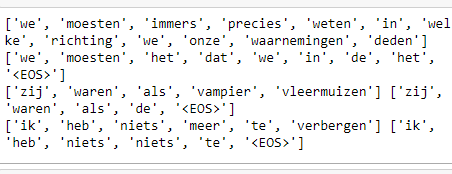
\includegraphics[width=7.8cm]{Screenshot (3).png}
    \label{Figure 1}
\end{figure}


\begin{thebibliography}{}

\bibitem[\protect\citename{Bahdanau \bgroup et al.\egroup}2014]{Bahdanau:2014}
D. Bahdanau, K. Cho, Y. Bengio.
\newblock 2014.
\newblock {\em Neural machine translation by jointly learning to align and translate.}
\newblock Retrieved from the arXiv database.

\bibitem[\protect\citename{Cho \bgroup et al.\egroup}2014]{Cho:2014}
K. Cho, B. van Merrienboer, C. Gulcehre, D. Bahdanau, F. Bougares, H. Schwenk, Y. Bengio.
\newblock 2014.
\newblock {\em Learning phrase representations using RNN encoder-decoder for statistical machine translation.}
\newblock Retrieved from the arXiv database.

\bibitem[\protect\citename{Jaeger}2002]{Jaeger:2002}
H. Jaeger.
\newblock 2002.
\newblock {\em A tutorial on training recurrent neural networks, covering BPPT, RTRL, EKF and the "echo state network" approach}

\bibitem[\protect\citename{Kalchbrenner \bgroup et al.\egroup}2013]{Kalchbrenner:2013}
N. Kalchbrenner, Phil Blunsom
\newblock 2013.
\newblock {\em Recurrent Continuous Translation Models}
\newblock Association for Computational Linguistics

\bibitem[\protect\citename{Papineni \bgroup et al.\egroup}2002]{Papineni:2002}
K. Papineni, S. Roukos, T. Ward, W. Zhu.
\newblock 2002
\newblock {\em BLEU: a Method for Automatic Evaluation of Machine Translation}
\newblock Proceedings of the 40th Annual Meeting of the Association for Computational Linguistics (ACL)

\bibitem[\protect\citename{PyTorch}2017]{PyTorch:17}
\newblock {\em NLP From Scratch: Translation with a Sequence to Sequence Network and Attention}

\bibitem[\protect\citename{Sutskever \bgroup et al.\egroup}2014]{Sutskever:2014}
I. Sutskever, O. Vinyals, Q. Le.
\newblock 2014.
\newblock {\em Sequence to sequence learning with neural networks.}
\newblock Retrieved from the arXiv database.

\end{thebibliography}

\end{document}
